%%%%%%%%%%%%%%%%%%%%%%%%%%%%%%%%%%%%%%%%%%%%%%%%%%%%%%%%%%%%%%%%%%%%%%%%%%%%%
\documentclass[10pt]{beamer}
\usefonttheme{professionalfonts}
\mode<presentation>
%%%%%%%%%%%%%%%%%%%%%%%%%%%%% THEME
{
%\usetheme{Antibes}
\usetheme{CambridgeUS}
\setbeamercovered{transparent}
\setbeamertemplate{frametitle}[default][center]
}

\newcommand\Switch{0}
\newcommand\SecInHead{%
  \ifthenelse{\equal{\Switch}{1}}
    {\thesection.}{}}
\newcommand\SubSecInHead{%
  \ifthenelse{\equal{\Switch}{1}}
    {\thesubsection. }{}}
\newcommand\RealSubSecInHead{%
  \ifthenelse{\equal{\thesubsection}{0}}
    {}{\SecInHead\SubSecInHead}}

\usepackage{subfigure}
\usepackage{amsmath,epsfig,graphicx,setspace,url,float,enumerate}
\usepackage{arydshln}%for horizontal dash lines...
\usepackage{graphicx}
\usepackage{booktabs}
\defbeamertemplate{itemize item}{image}{\small\includegraphics[height=1.5ex]{red-bullet-on-white.ps}}
\defbeamertemplate{itemize subitem}{image}{\scriptsize\includegraphics[height=1.5ex]{green-bullet-on-white.ps}}
\defbeamertemplate{itemize subsubitem}{image}{\scriptsize\includegraphics[height=1.5ex]{yellow-bullet-on-white.ps}}
\setbeamertemplate{itemize item}[image]
\setbeamertemplate{itemize subitem}[image]
\setbeamertemplate{itemize subsubitem}[image]
\setbeamertemplate{bibliography item}[text]
%%%%%%%%%%%%%%%%%%%%%%%%%%%%%%%%%%%%%%%%%%%%%%%%%%%%%%%%%%%%%%%%%%%%%%%%%%%%%%%%%%%%%%%%%%%%%%%%%%%%%%%%%%%%%%%%
%%%%%%%%%%%%%%%%%%%%%%%%%%%%%%%%%%%%%%%%%%%%%%%%%%%%%%%%%%%%%%%%%%%%%%%%%%%%%%%%%%%%%%%%%%%%%%%%%%%%%%%%%%%%%%%%
\title { Cascaded LQR Control for Missile Roll Autopilot}
\author{D Viswanath and TS Chandar}
%\institute[IIT Guwahati]{IIT Guwahati}
\date{\today}
\begin{document}
%%%%%%%%%%%%%%%%%%%%%%%%%%%%%%%%%%%%%%%%%%%%%%%%%%%%%%%%%%%%%%%%%%%%%%%%%%%%%%%%%%%%%%%%%%%%%%%%%%%%%%%%%%%%%%%%
\section{IC4 Conference}

\begin{frame}
\frametitle{\textbf{Cascaded LQR Control for Missile Roll Autopilot}}
\begin{center}
\vspace{0.5cm}
{\small{\sf \sf \textbf{D Viswanath}}}\\[0.5ex]
{\small{\sf \sf \textbf{\color{gray}Dept of Electronics \& Electrical Engg,\\IIT Guwahati}}}\\[0.5ex]
\vspace{.5cm}
{\small{\sf \sf \textbf{TS Chandar}}}\\
{\small{\sf \sf \textbf{\color{gray}Dept of Electronics \& Communication Engg, \\PES University,\\Bengaluru}}}\\[0.5ex]
\vspace{-.5cm}
%{\small{\sf \sf \textbf{Supervisor}}}\\[0.5ex]
%{\small{\sf \sf \textbf{S. R. M. Prasanna}}}\\[1ex]
%{\small {\sf \sf \textbf{\color{gray}{Department of Electronics and Electrical Engineering}}}} \\[.5ex]
%{\small{\sf \sf \textbf{\color{gray}Indian Institute of Technology Guwahati}}}  \\[.5ex]
%%%{\small{\sf \sf \textbf{\color{gray}December, 2011}}}
\end{center}
\end{frame}
%%%%%%%%%%%%%%%%%%%%%%%%%%%%%%%%%%%%%%%%%%%%%%%%%%%%%%%%%%%%%%%%%%%%%%%%%%%%%%%%%%%%%%%%%%%%%%%%%%%%%%%%%%%%%%%%
%%%            Slides
%%%%%%%%%%%%%%%%%%%%%%%%%%%%%%%%%%%%%%%222222222%%%%%%%%%%%%%%%%%%%%%%%%%%%%%%%%%%%%%%%%%%%%%%%%%%%%%%%%%%%%%%%%%%%%%%%%%

\subsection{ Overview}
\begin{frame}
\frametitle{Overview}
\renewcommand{\baselinestretch}{1}
\begin{itemize}
\item Introduction \bigskip
\item Literature Survey \bigskip
\item Motivation \bigskip
\item Missile Roll Autopilot Design \bigskip
\begin{itemize}
 \item Background \smallskip
 \item Design of Missile Autopilot with Cascaded LQR \smallskip
  \item Simulation Results and Analysis \bigskip
 \end{itemize}
 \item Conclusion \bigskip
\end{itemize}
\end{frame}
%%%%%%%%%%%%%%%%%%%%%%%%%%%%%%%%%%%%%%%%%%%%%%%%%%%%%%%%%%%%%%%%%%%%%%%%%%%%%%

%%%%%%%%%%%%%%%%%%%%%%%%%%%%%%%%%%%%%%%222222222%%%%%%%%%%%%%%%%%%%%%%%%%%%%%%%%%%%%%%%%%%%%%%%%%%%%%%%%%%%%%%%%%%%%%%%%%

\section{ Introduction}
%\subsection{ Roll Autopilot Design}
\begin{frame}
\frametitle{Introduction}
\begin{itemize}
\item  Modern missiles are required to be very agile and stable platforms. \bigskip
\item  The main aim of the roll autopilot in a cruciform cartesian controlled missile is to maintain roll angle zero thus ensuring that the dynamics in the three dimensions of roll, pitch and yaw channels are decoupled. \bigskip
\item  Decoupling of the dynamics helps in formulating simple simultaneous equations for the roll, pitch and yaw channels respectively and makes computations
simpler and implementation easier. \bigskip
\end{itemize}
\end{frame}
%%%%%%%%%%%%%%%%%%%%%%%%%%%%%%%%%%%%%%%%%%%%%%%%%%%%%%%%%%%%%%%%%%%%%%%%%%%%%%
\begin{frame}
\frametitle{Introduction}
\begin{itemize}
\item  Missile roll autopilots were first designed using classical control approaches. \bigskip
\item  Classical control was effective for lower order model of roll autopilot. \bigskip
\item  Optimal control as a modern control system design approach when used in aerospace applications can meet the requirements of fast response with minimum settling time and good stability characteristics. \bigskip
\item  Linear Quadratic Regulator is a ubiquitous optimal controller which can be used effectively in the design of a missile roll autopilot. \bigskip
\end{itemize}
\end{frame}
%%%%%%%%%%%%%%%%%%%%%%%%%%%%%%%%%%%%%%%%%%%%%%%%%%%%%%%%%%%%%%%%%%%%%%%%%%%%%%%%%%
\section{ Literature Survey}
\subsection{Classical Control Approach}
\begin{frame}
\frametitle{Literature Survey}
\begin{itemize}
 \item Missile roll autopilots were first designed using classical control approach like proportional-integral feedback control.Instability in design due to inclusion of second order actuator dynamics was overcome using lag-lead compensation \cite{garnell}. \bigskip
 \item Optimal control approach combined with classical approach for design of robust missile roll autopilots was first discussed in \cite{zarchannesline81}. \bigskip
 \item \cite{zarchannesline1984} discusses the design of an optimal controller using a computer program called OPTSYS (Optimum System Synthesis) \bigskip
\end{itemize}
\vspace{.5cm}
\footnoterule
\tiny {\cite{garnell} P. Garnell, [1980] ``Guided Weapon Control Systems'',2nd ed., Pergamon Press} \\
\tiny {\cite{zarchannesline81} Zarchan et al [1981] ``Combined Optimal/Classical Approach to Robust Missile Autopilot Design'',Journal of Guidance and Control} \\
\tiny {\cite{zarchannesline1984} FW Nesline and Zarchan [1984] ``Why Modern Controllers can go Unstable in Practice'',Journal of Guidance}
\end{frame}
%% %%%%%%%%%%%%%%%%%%%%%%%%%%%%%%%%%%%%%%%%%%%%%%%%%%%%%%%%%%%%%%%%%%%%%%%%%%%%%%
%\subsection{Modern Control Approach}
%\begin{frame}
%\frametitle{Literature Survey}
%\begin{itemize}
% \item Optimal control approach combined with classical approach for design of robust missile roll autopilots was first discussed in \cite{zarchannesline81}. \bigskip
% \item \cite{zarchannesline1984} discusses the design of an optimal controller using a computer program called OPTSYS (Optimum System Synthesis)\bigskip
% \item In \cite{briantsourdos2001}, the authors have provided an overview of modern missile flight control design and discussed various modern control approaches like robust gain scheduling, linear parameter varying control design, nonlinear dynamic inversion and optimal control using linear quadratic control, genetic algorithm or $H_2/H_{\infty}$. \bigskip
%\end{itemize}
%\vspace{.5cm}
%\footnoterule
%\tiny {\cite{zarchannesline81} Zarchan et al [1981] ``Combined Optimal/Classical Approach to Robust Missile Autopilot Design'',Journal of Guidance and Control} \\
%\tiny {\cite{zarchannesline1984} FW Nesline and Zarchan [1984] ``Why Modern Controllers can go Unstable in Practice'',Journal of Guidance} \\
%\tiny {\cite{briantsourdos2001} B White and A Tsourdos [2001] ``Modern Missile Flight Control Design: An Overview'', Proc. of IFAC Symposium}
%\end{frame}
% %%%%%%%%%%%%%%%%%%%%%%%%%%%%%%%%%%%%%%%%%%%%%%%%%%%%%%%%%%%%%%%%%%%%%%%%%%%%%%
\subsection{LQR Approach}
\begin{frame}
\frametitle{Literature Survey}
\begin{itemize}
\item \cite{parkhi2010} proposes the design of a roll autopilot for the model including the rigid body dynamics and the actuator dynamics using Sliding Mode Control (SMC) technique with LQR optimization employed for design of sliding surface. \bigskip
 \item Robust missile roll autopilot design with application of linear quadratic regulator (LQR) for solving the combined dynamics of a flexible missile is discussed in \cite{talolekolhe2011}.  \bigskip
\end{itemize}
\vspace{.5cm}
\footnoterule
\tiny {\cite{parkhi2010} Parkhi et al [2010] ``Design of Roll Autopilot for a Tail Controlled Missile Using Sliding Mode Technique'',IEEE Workshop on Variable Structure Systems} \\
\tiny {\cite{talolekolhe2011} Talole et al [2011] ``Robust Autopilot Design for Tactical Missiles'', Journal of Guidance, Control, and Dynamics}
\end{frame}
% %%%%%%%%%%%%%%%%%%%%%%%%%%%%%%%%%%%%%%%%%%%%%%%%%%%%%%%%%%%%%%%%%%%%%%%%%%%%%%
\subsection{Cascaded LQR Approach}
\begin{frame}
\frametitle{Literature Survey}
\begin{itemize}
 \item In \cite{gattami2005}, the authors discuss the problem of linear quadratic regulator (LQR) performance for cascade control structures of series coupled systems and obtain the necessary and sufficient condition for the linear quadratic performance of a cascade control structure to achieve the same performance as any given centralized LQR. \bigskip
\item Cascaded control has found applications in acceleration and displacement control of an electrodynamic shaker \cite{fujita2006}, evolutionary optimization of cascaded industrial hydraulic valves \cite{hoffman2007}, and optimal control of heavy vehicle formations \cite{gattami2011}. \bigskip
\end{itemize}
\vspace{.5cm}
\footnoterule
\tiny {\cite{gattami2005} A Gattami and A Rantzer [2005] ``Linear Quadratic Performance Criteria for Cascade Control'',Proc of IEEE/ECC Conference} \\
\tiny {\cite{fujita2006} Y Uchiyama and M Fujita,[2006] ``Robust Acceleration and Displacement Control of Electrodynamic Shaker,''IEEE Conference}\\
\tiny {\cite{hoffman2007} Krettek et al [2007] ``Evolutionary Hardware-in-the-loop Optimization of a Controller for Hydraulic Valves'',IEEE/ASME International Conference} \\
\tiny {\cite{gattami2011} Gattami et al [2011] ``Suboptimal Decentralized Controller Design for Chain Structures: Applications to Vehicle Formations '', IEEE Conference}
\end{frame}
%%%%%%%%%%%%%%%%%%%%%%%%%%%%%%%%%%%%%%%%%%%%%%%%%%%%%%%%%%%%%%%%%%%%%%%%%%%%%%%
%%%%%%%%%%%%%%%%%%%%%%%%%%%%%%%%%%%%%%%%%%%%%%%%%%%%%%%%%%%%%%%%%%%%%%%%%%%%%%%%%%%%%%%%%%%%%%%%%%%%%%%%%%%%%%%%%%%%%%%%%%%%%%%%%%%%%%%%%%%%%%%%%%%%%%%%%%%%%%%%%%%%%%
\section{ Motivation}
\subsection{Advantages and Disadvantages}
\begin{frame}
\frametitle{Motivation}
\begin{itemize}
 \item Advantages: \bigskip
 \begin{itemize}
    \item In cascaded LQR based approach the states can be {\color{blue}measured} as they are physical quantities. \smallskip
    \item Whereas when centralized LQR is used, the higher order states are obtained by differentiation of output and can only be {\color{blue}estimated} since they are not physically quantifiable.  \bigskip
 \end{itemize}
 \item Disadvantages: \smallskip
 \begin{itemize}
 \item {\color{blue}Flexible body dynamics} cannot be included in this approach since they cannot be measured. \bigskip
\end{itemize}
\end{itemize}

\vspace{.4cm}
\end{frame}
%%%%%%%%%%%%%%%%%%%%%%%%%%%%%%%%%%%%%%%%%%%%%%%%%%%%%%%%%%%%%%%%%%%%%%%%%%%%%%%%%%%%%%%%%%%%%%%%%%%%%%%%%%%%%%%%%%%%%%%%%%%%%%%%%%%%%%%%%%%%%%%%%%%%%%%%%%%%%%%%%%%%%
\section{ Missile Roll Autopilot Design}
\subsection{Background}
\begin{frame}
\frametitle{Cascaded LQR}
The realistic model of the roll autopilot considering the missile airframe, actuator,and gyro dynamics is as shown in block diagram below
\begin{figure}[h]
\begin{center}
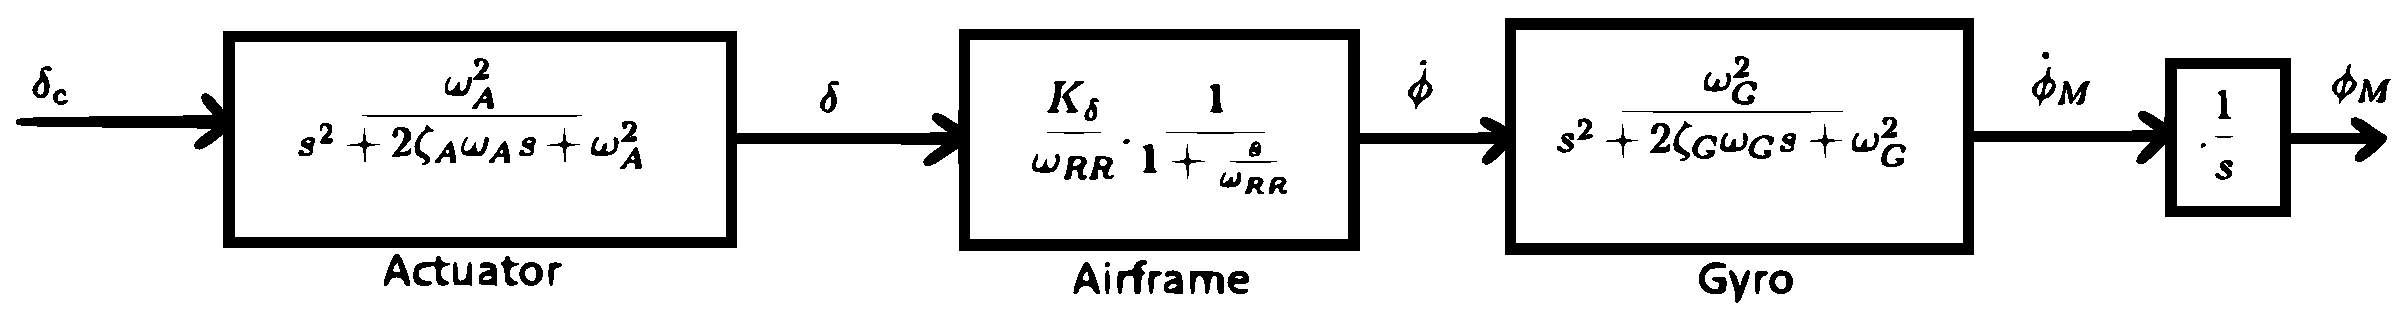
\includegraphics[width=9.0cm,height=2.5cm]{BlockDiaLQRs14.eps}
\vspace{-0.2cm}
\caption{\bf{Missile Roll Autopilot \cite{zarchannesline81}\cite{zarchannesline1984}}} \label{Cascade14}
\end{center}
\vspace{-0.5cm}
\end{figure}
\vspace{.5cm}
\footnoterule
\tiny {\cite{zarchannesline81} Zarchan et al [1981] ``Combined Optimal/Classical Approach to Robust Missile Autopilot Design'',Journal of Guidance and Control} \\
\tiny {\cite{zarchannesline1984} FW Nesline and Zarchan [1984] ``Why Modern Controllers can go Unstable in Practice'',Journal of Guidance} \\
%where
%\begin{itemize}
% \item $\phi_M$ is measured roll angle and $\delta_c$ is the fin deflection command,
%  \item $K_\delta$ is the fin effectiveness and $\omega_{RR}$ is the roll rate bandwidth,
% \item $\omega_A$ is the actuator bandwidth and $\zeta_A$ is the actuator damping,
% \item  $\omega_G$ is the rate gyro bandwidth and $\zeta_G$ is the rate gyro damping,
% \item $\omega_l$ is the flexible body dynamics bandwidth and $\zeta_l$ is the flexible body dynamics damping constant.
%\end{itemize}

\vspace{.4cm}
\end{frame}
%%%%%%%%%%%%%%%%%%%%%%%%%%%%%%%%%%%%%%%%%%%%%%%%%%%%%%%%%%%%%%%%%%%%%%%%%%%%%%%%%%%%
\begin{frame}
\frametitle{Background}
The transfer function for this model is given by
\begin{eqnarray}
\frac{\phi_M}{\delta_c}&=&\frac{\omega_A^2}{s^2+2\zeta_A \omega_A s+\omega_A^2}\\\nonumber
&\times&\bigg[\frac{K_\delta}{\omega_{RR}}.\frac{1}{(1+\frac{s}{\omega_{RR}})}\bigg]\\\nonumber
&\times&\frac{\omega_G^2}{s^2+2\zeta_G \omega_G s+\omega_G^2}.\frac{1}{s}\label{RollAPlqr5}
\end{eqnarray}
where
\begin{itemize}
 \item $\phi_M$ is measured roll angle and $\delta_c$ is the fin deflection command,
  \item $K_\delta$ is the fin effectiveness and $\omega_{RR}$ is the roll rate bandwidth,
 \item $\omega_A$ is the actuator bandwidth and $\zeta_A$ is the actuator damping,
 \item  $\omega_G$ is the rate gyro bandwidth and $\zeta_G$ is the rate gyro damping,
\end{itemize}

\vspace{.4cm}
\end{frame}
%
%%%%%%%%%%%%%%%%%%%%%%%%%%%%%%%%%%%%%%%%%%%%%%%%%%%%%%%%%%%%%%%%%%%%%%%%
\begin{frame}
\frametitle{Background}
\begin{itemize}
 \item Most classical control approaches \cite{garnell} omit the higher order dynamics of the second order gyro.
  \item In recent times, with advent of modern state space approach, strategies like optimal control based on LQR \cite{zarchannesline81},\cite{zarchannesline1984} and nonlinear control laws like Extended State Observer (ESO) \cite{talolekolhe2011} which include these higher order dynamics have been proposed.
\end{itemize}
\vspace{.5cm}
\footnoterule
\tiny {\cite{garnell} P. Garnell, [1980] ``Guided Weapon Control Systems'',2nd ed., Pergamon Press} \\
\tiny {\cite{zarchannesline81} Zarchan et al [1981] ``Combined Optimal/Classical Approach to Robust Missile Autopilot Design'',Journal of Guidance and Control} \\
\tiny {\cite{zarchannesline1984} FW Nesline and Zarchan [1984] ``Why Modern Controllers can go Unstable in Practice'',Journal of Guidance} \\
\tiny {\cite{talolekolhe2011} Talole et al [2011] ``Robust Autopilot Design for Tactical Missiles'', Journal of Guidance, Control, and Dynamics}

\vspace{.4cm}
\end{frame}
%
%%%%%%%%%%%%%%%%%%%%%%%%%%%%%%%%%%%%%%%%%%%%%%%%%%%%%%%%%%%%%%%%%%%%%%%%
\subsection{Cascaded LQR}
\begin{frame}
\frametitle{Cascaded LQR}
Let us consider the block diagram for the realistic model of the roll autopilot again
\begin{figure}[h]
\begin{center}
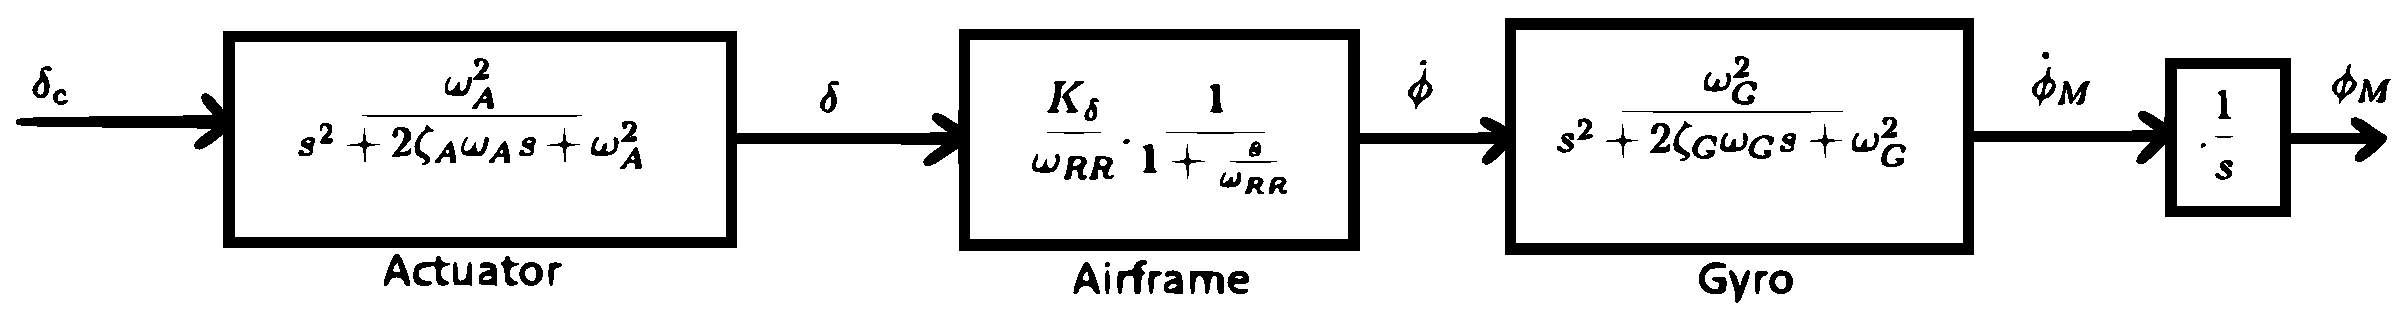
\includegraphics[width=8.4cm,height=2.0cm]{BlockDiaLQRs14.eps}
\vspace{-0.2cm}
\caption{\bf{Missile Roll Autopilot}} \label{Cascade14}
\end{center}
\vspace{-0.5cm}
\end{figure}

In the cascaded form
\begin{itemize}
\item The first block is represented by system $\Sigma_4$ with input $U_4=\delta_C$ and output $Y_4=\delta$,
\item The second block is represented by system $\Sigma_3$ with input $U_3=Y_4=\delta$ and output $Y_3=\dot \phi$,
\item The third block is represented by system $\Sigma_2$ with input $U_2=Y_3=\dot \phi$ and output $Y_2=\dot \phi_M$, and
\item The fourth block is represented by system $\Sigma_1$ with input $U_1=Y_4=\dot \phi_M$ and output $Y_1=\phi_M$.
\end{itemize}
\vspace{.4cm}
\end{frame}
%
%%%%%%%%%%%%%%%%%%%%%%%%%%%%%%%%%%%%%%%%%%%%%%%%%%%%%%%%%%%%%%%%%%%%%%%%
\begin{frame}
\frametitle{Cascaded LQR}
Let the state space form for each block be given by
\begin{itemize}
 \item
 \begin{eqnarray}
\dot X_4&=&A_4 X_4+B_4 U_4\\\nonumber
Y_4&=&C_4 X_4\label{RollAPclqr11a}
\end{eqnarray}
  \item
  \begin{eqnarray}
\dot X_3&=&A_3 X_3+B_3 U_3\\\nonumber
Y_3&=&C_3 X_3\label{RollAPclqr12a}
\end{eqnarray}
 \item
 \begin{eqnarray}
\dot X_2&=&A_2 X_2+B_2 U_2\\\nonumber
Y_2&=&C_2 X_2\label{RollAPclqr13a}
\end{eqnarray}
 \item
 \begin{eqnarray}
\dot X_1&=&A_1 X_1+B_1 U_1\\\nonumber
Y_1&=&C_1 X_1\label{RollAPclqr13b}
\end{eqnarray}
\end{itemize}

\vspace{.4cm}
\end{frame}
%
%%%%%%%%%%%%%%%%%%%%%%%%%%%%%%%%%%%%%%%%%%%%%%%%%%%%%%%%%%%%%%%%%%%%%%%%
\begin{frame}
\frametitle{Cascaded LQR}
The state space representation of the cascaded systems $\Sigma_1$, $\Sigma_2$, $\Sigma_3$ and $\Sigma_4$ with $U_c=U_4$ can be written as a larger system $\Sigma_c$ given by
\begin{eqnarray}
\dot X_c&=&\textbf{A}_c X+\textbf{B}_c U_c\\
Y_c&=&\textbf{C}_c X_c\label{RollAPclqr14}
\end{eqnarray}
where
$$X_c=[\delta~~\dot \delta~~\dot \phi~~\dot \phi_M~~\ddot \phi_M~~\phi_M]^T$$

\begin{equation}
\textbf{A}_c=\begin{bmatrix} \textbf{A}_1~~~~\textbf{B}_1 \textbf{C}_2~~~~~0~~~~~~~0~~~~~~~0~~\\
0~~~~~~~\textbf{A}_2~~~~~~\textbf{B}_2 \textbf{C}_3~~~0~~~~~~~0~~\\
0~~~~~~~~0~~~~~~~~0~~~~~~~\textbf{A}_3~~~\textbf{B}_3 \textbf{C}_4\\
0~~~~~~~~0~~~~~~~~0~~~~~~~~0~~~~~~\textbf{A}_4~\end{bmatrix}\label{RollAPclqr15}
\end{equation}
and
\begin{equation}
\textbf{B}_c=\begin{bmatrix}0\\0\\0\\0\\\textbf{B}_4\end{bmatrix}~;~\textbf{C}_c=\bigg[ \textbf{C}_1~~0~~0~~0~~0~~0 \bigg]\label{RollAPclqr16}
\end{equation}

\vspace{.4cm}
\end{frame}
%%%%%%%%%%%%%%%%%%%%%%%%%%%%%%%%%%%%%%%%%%%%%%%%%%%%%%%%%%%%%%%%%%%%%%%%%%%%%%%%%%%%%%
%%%%%%%%%%%%%%%%%%%%%%%%%%%%%%%%%%%%%%%%%%%%%%%%%%%%%%%%%%%%%%%%%%%%%%%%
\begin{frame}
\frametitle{Cascaded LQR}
The linear quadratic regulator for $\Sigma_c$ is designed to minimize the performance index given by
\begin{equation}
J_c=\frac{1}{2} \int_0^\infty \bigg[ X_c^T\textbf{Q}_c X_c+U_c^T \textbf{R}_c U_c \bigg]dt \label{RollAPoptimal5a}
\end{equation}
The control law is given by
\begin{equation}
U_c=-\textbf{L}_c X_c\label{RollAPoptimal6a}
\end{equation}
where $\textbf{L}_c=\textbf{R}_c^{-1}\textbf{B}_c^T\textbf{P}_c$ and $\textbf{P}_c$ is the solution to the algebraic matrix Riccati equation given by
\begin{equation}
\textbf{P}_c \textbf{A}_c+\textbf{A}_c^T\textbf{P}_c-\textbf{P}_c \textbf{B}_c \textbf{R}_c^{-1}\textbf{B}_c^T\textbf{P}_c+\textbf{Q}_c=0\label{RollAPoptimal7a}
\end{equation}

The matrices $\textbf{Q}_c$ and $\textbf{R}_c$ are chosen to be positive definite.
\vspace{.4cm}
\end{frame}
%%%%%%%%%%%%%%%%%%%%%%%%%%%%%%%%%%%%%%%%%%%%%%%%%%%%%%%%%%%%%%%%%%%%%%%%%%%%%%%%%%%%%%%%%%%%
\section{Simulation Results}
\subsection{Simulation Parameters}
\begin{frame}
\frametitle{Simulation Parameters}
The design values in \cite{zarchannesline81} for the gains and bandwidths which were used in the simulations are given in table below.
\begin{table}[!t]
% increase table row spacing, adjust to taste
\renewcommand{\arraystretch}{1.5}
% if using array.sty, it might be a good idea to tweak the value of
% \extrarowheight as needed to properly center the text within the cells
\caption{Simulation Parameters}
\label{table_rollAP}
\centering
% Some packages, such as MDW tools, offer better commands for making tables
% than the plain LaTeX2e tabular which is used here.
\begin{tabular}{|c||c| |c|}
\hline
Parameter & Name & Value\\
\hline
$\omega_{RR}$ & Roll Rate Bandwidth & $2$ rad/s\\
\hline
$K_\delta$ & Fin effectiveness & $9000$ $\frac{1}{s^2}$\\
\hline
$\omega_A$ & Actuator Bandwidth & $100$ rad/s\\
\hline
$\zeta_A$ & Actuator Damping & $0.65$\\
\hline
$\omega_G$ & Gyro Bandwidth & $200$ rad/s\\
\hline
$\zeta_G$ & Gyro Damping & $0.5$\\
\hline
\end{tabular}
\end{table}
\vspace{.5cm}
\footnoterule
\tiny {\cite{zarchannesline81} Zarchan et al [1981] ``Combined Optimal/Classical Approach to Robust Missile Autopilot Design'',Journal of Guidance and Control}
\end{frame}
%%%%%%%%%%%%%%%%%%%%%%%%%%%%%%%%%%%%%%%%%%%%%%%%%%%%%%%%%%%%%%%%%%%%%%%%%%%%%%%%%%%%%%%%%%%%%%%%%%%%
\begin{frame}
\frametitle{Simulation Parameters}
The maximum values for a safe and controlled launch used in \cite{zarchannesline1984} are given in table below.

\begin{table}[!t]
% increase table row spacing, adjust to taste
\renewcommand{\arraystretch}{1.6}
% if using array.sty, it might be a good idea to tweak the value of
% \extrarowheight as needed to properly center the text within the cells
\caption{Maximum Values for Desired LQR Performance}
\label{table_rollAPlqr}
\centering
% Some packages, such as MDW tools, offer better commands for making tables
% than the plain LaTeX2e tabular which is used here.
\begin{tabular}{|c||c| |c|}
\hline
Parameter & Name & Value\\
\hline
$\phi_{MX}$ & Maximum Desired Roll Angle & $0.174$ rad\\
\hline
$\dot \phi_{MX}$ & Maximum Desired Roll Rate & $5.23$ rad/sec\\
\hline
$\delta_{CMX}$ & Maximum Desired Fin Deflection & $0.524$ rad\\
\hline
\end{tabular}
\end{table}
\vspace{.5cm}
\footnoterule
\tiny {\cite{zarchannesline1984} FW Nesline and Zarchan [1984] ``Why Modern Controllers can go Unstable in Practice'',Journal of Guidance}
\end{frame}
%%%%%%%%%%%%%%%%%%%%%%%%%%%%%%%%%%%%%%%%%%%%%%%%%%%%%%%%%%%%%%%%%%%%%%%%%%%%%%%%%%%%%%%%%%%%%%%%%%%%
\begin{frame}
\frametitle{Simulation Parameters}
The matrices $\textbf{Q}_c$ and $\textbf{R}_c$ are chosen as
\begin{equation}
\textbf{Q}_c=\begin{bmatrix}\frac{1}{\phi_{MX}^2}~~~~~0~~~~~0~~~~~0~~~~~0~~~~~0~~~\\
~~0~~~~~\frac{1}{\dot \phi_{MX}^2}~~~0~~~~~0~~~~~0~~~~~0~~~\\
~~0~~~~~~~0~~~~~0~~~~~0~~~~~0~~~~~0~~~\\
~~0~~~~~~~0~~~~~0~~~~~0~~~~~0~~~~~0~~~\\
~~0~~~~~~~0~~~~~0~~~~~0~~~~~0~~~~~0~~~\\
~~0~~~~~~~0~~~~~0~~~~~0~~~~~0~~~~~0~~~\end{bmatrix}\label{RollAPoptimal22}
\end{equation}
and
\begin{equation}
\textbf{R}_c=\frac{1}{\delta_{CMX}^2}\label{RollAPoptimal23}
\end{equation}

Solving equation (\ref{RollAPoptimal7a}), the controller gains are computed as $$\textbf{L}_c=[3.0115~~0.0102~~0.000013~~0.1348~~8.985~~0.0313]$$

\end{frame}
%%%%%%%%%%%%%%%%%%%%%%%%%%%%%%%%%%%%%%%%%%%%%%%%%%%%%%%%%%%%%%%%%%%%%%%%%%%%%%%%%%%%%%%%%%%%%%%%%%%%%%%%%%%
\subsection{Results}
\frametitle{Simulation Results}
\begin{frame}
\frametitle{Simulation Results}
For a comparison with the sliding mode control based roll autopilot in \cite{parkhi2010} with nominal parameters,
\begin{itemize}
\item The initial values in measured roll angle and roll rate are assumed to be $-0.7~rad$ and $+0.7~rad/s$
\item All other initial conditions are assumed to be zero, giving $X_c(0)=[0~~0~~0~~0.7~~0~~-0.7]^T$.
\item The time domain specifications from \cite{parkhi2010} are rise time not more than $50~ms$, settling time less than $200~ms$ and peak overshoot($M_p$) below $15$\%.
\end{itemize}
\vspace{.5cm}
\footnoterule
\tiny {\cite{parkhi2010} Parkhi et al [2010] ``Design of Roll Autopilot for a Tail Controlled Missile Using Sliding Mode Technique'',IEEE Workshop on Variable Structure Systems}
\end{frame}
%%%%%%%%%%%%%%%%%%%%%%%%%%%%%%%%%%%%%%%%%%%%%%%%%%%%%%%%%%%%%%%%%%%%%%%%%%%%%%%%%%%%%%%%%%%%%%%%%%%%%%%%%%
\begin{frame}
\frametitle{Simulation Results}
Figure below shows the measured roll angle ($\phi_M$). The response obtained is similar to the SMC Roll Autopilot i.e., dead-beat type with no overshoot and settling time approximately $180~ms$.
\begin{figure}[!h]
\begin{center}
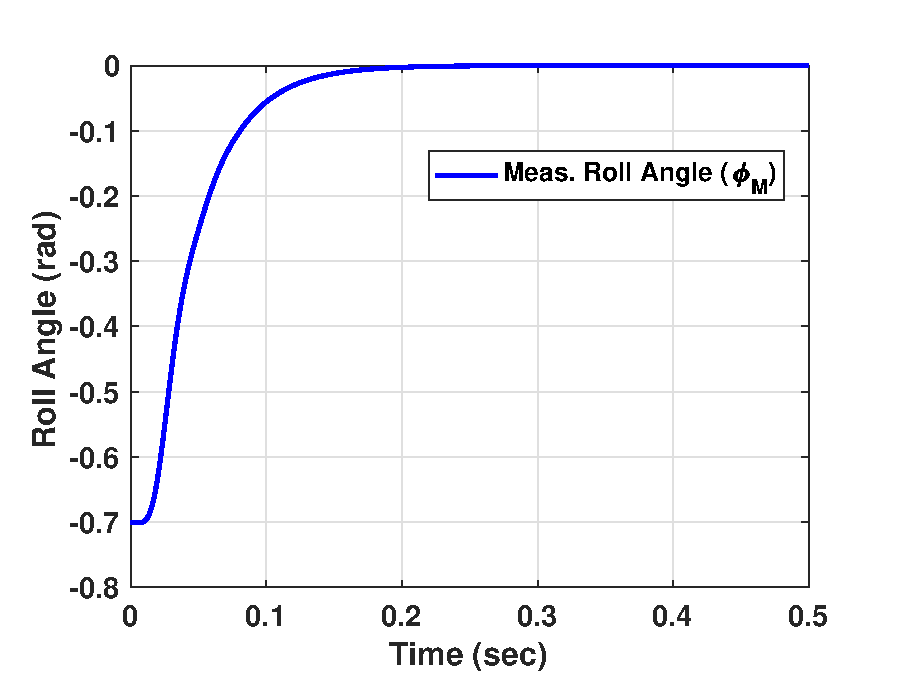
\includegraphics[width=6cm,height=3.0cm]{CascRollAP61.eps}
\vspace{-0.2cm}
\caption{\bf{Measured Roll Angle.}} \label{rollAP13}
\end{center}
\vspace{-0.5cm}
\end{figure}

\end{frame}
%%%%%%%%%%%%%%%%%%%%%%%%%%%%%%%%%%%%%%%%%%%%%%%%%%%%%%%%%%%%%%%%%%%%%%%%%%%%%%%%%%%%%%%%%%%%%%%%%%%%%%%%%%
\begin{frame}
\frametitle{Simulation Results}
Figure below shows the actual roll rate ($\dot \phi$) and measured roll rate ($\dot \phi_M$) respectively.  The settling time is approximately $180~ms$; rise time is less than $50~ms$. The initial lag in the actual and measured roll rates is due to the second order gyro dynamics. The lag is negligible after $100~ms$.

\begin{figure}[!h]
\begin{center}
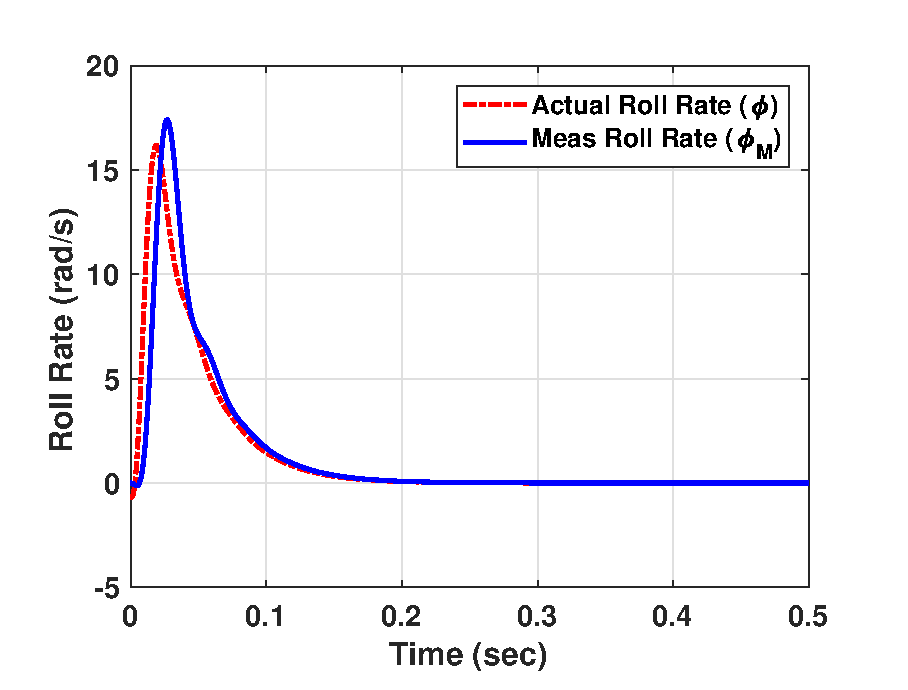
\includegraphics[width=6cm,height=3.0cm]{CascRollAP62.eps}
\vspace{-0.2cm}
\caption{\bf{Roll Rate.}} \label{rollAP12}
\end{center}
\vspace{-0.5cm}
\end{figure}

\end{frame}
%%%%%%%%%%%%%%%%%%%%%%%%%%%%%%%%%%%%%%%%%%%%%%%%%%%%%%%%%%%%%%%%%%%%%%%%%%%%%%%%%%%%%%%%%%%%%%%%%%%%%%%%%%
\begin{frame}
\frametitle{Simulation Results}
Figure below shows the commanded fin deflection ($\delta_C$) and the actual fin deflection ($\delta$). The observed maximum fin deflection in both cases is well within the limits of the desired maximum fin deflection given in Table II.
%
\begin{figure}[!h]
\begin{center}
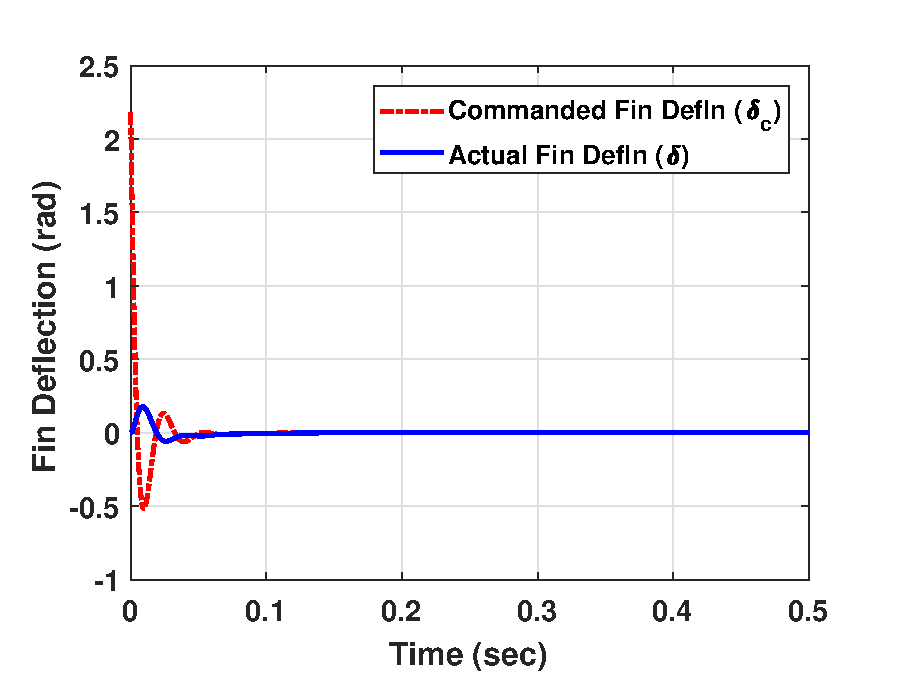
\includegraphics[width=6cm,height=3.0cm]{CascRollAP63a.eps}
\vspace{-0.2cm}
\caption{\bf{Fin Deflection}} \label{rollAP11}
\end{center}
\vspace{-0.5cm}
\end{figure}

\end{frame}
%%%%%%%%%%%%%%%%%%%%%%%%%%%%%%%%%%%%%%%%%%%%%%%%%%%%%%%%%%%%%%%%%%%%%%%%%%%%%%%%%%%%%%%%%%%%%%%%%%%%%%%%%%
\begin{frame}
\frametitle{Simulation Results}
A comparison of the time response of SMC Roll Autopilot from \cite{parkhi2010} and Cascaded LQR (CLQR) is given in Table below.

\begin{table}[!h]
\renewcommand{\arraystretch}{1.6}
\caption{COMPARATIVE TIME RESPONSE}
\begin{center}
\begin{tabular}{|c|c|c||c|c|c|}
\hline
\multicolumn{3}{|c|}{\textbf{SMC Autopilot}} &\multicolumn{3}{|c|}{\textbf{CLQR Autopilot}}\\
\hline
\hline
$M_p$ & $||\dot \phi_M||_\infty$ & $||\delta||_\infty$ & $M_p$ & $||\dot \phi_M||_\infty$ & $||\delta||_\infty$
\\
\hline
(\%) & ($deg/s$) & ($deg$) & (\%) & ($deg/s$) & ($deg$) \\
\hline
$1.00$ & $922.14$ & $10.10$ & $1.00$ & $996.775$ & $10.07$\\
\hline
%\multicolumn{4}{l}{$^{\mathrm{a}}$Sample of a Table footnote.}
\end{tabular}
\label{tab1}\\
\vspace{.5cm}
\footnoterule
\tiny {\cite{parkhi2010} Parkhi et al [2010] ``Design of Roll Autopilot for a Tail Controlled Missile Using Sliding Mode Technique'',IEEE Workshop on Variable Structure Systems}
\end{center}
\end{table}

\end{frame}
%%%%%%%%%%%%%%%%%%%%%%%%%%%%%%%%%%%%%%%%%%%%%%%%%%%%%%%%%%%%%%%%%%%%%%%%%%%%%%%%%%%%%%%%%%%%%%%%%%%%%%%%%
\section{Conclusions and Future Scope}
\subsection{Conclusions}
\begin{frame}
 \frametitle{Conclusion}
 \begin{itemize}
 \item  Cascaded linear quadratic regulator is employed in the design of feedback controller for the missile roll autopilot considering the dynamics of second order actuator and second order gyro also in a realistic scenario.   \bigskip
  \item Simulations were carried out to verify the effectiveness of the controller and the time response was compared with SMC based roll autopilot. \bigskip
  \item The proposed cascaded LQR is not in a position to handle unmodeled flexible body dynamics which can be extended to parametric uncertainties and disturbances. \bigskip
  \end{itemize}
\end{frame}
%%%%%%%%%%%%%%%%%%%%%%%%%%%%%%%%%%%%%%%%%%%%%%%%%%%%%%%%%%%%%%%%%%%%%%%%%%%%%%%%%%%555%%%%%%%%%%%%%%%%%%%%%%%%%%%%%%%%%%%%%%%%%%%%%%%%%%%%%%%%%%%%%%%%%%%%%%%%%%%%%%%%%%555
\subsection{Future Scope}
\begin{frame}
 \frametitle{Future Scope}
 \begin{itemize}
 \item  The proposed cascaded LQR controller would be augmented with another controller for robustness in the presence of flexible body dynamics and model uncertainties. \bigskip
  \item Performance of this augmented controller will be compared with existing approaches.\bigskip
 \end{itemize}
\end{frame}
%%%%%%%%%%%%%%%%%%%%%%%%%%%%%%%%%%%%%%%%%%%%%%%%%%%%%%%%%%%%%%%%%%%%%%%%%%%%%%%%%%%%%%%%%%%%%%%%%%%%%%%%%%%%%%%%%%%%%%%%%%
\section{bibliography}
\setbeamertemplate{footline}{}
\begin{frame}[allowframebreaks]
\frametitle{References}

%\tiny{
%    \bibliographystyle{IEEEtran}
%
%	\tiny \bibliography{speech_synthesis}
%     }
\begin{thebibliography}{00}

\bibitem{garnell}
P. Garnell,
{``\it{ Guided Weapon Control Systems},''}\emph{2nd ed., Pergamon Press},
 Oxford, England, 1980.

\bibitem{zarchannesline81}
F. William Nesline, Brian H. Wells, and P. Zarchan,
``Combined Optimal/Classical Approach to Robust Missile Autopilot Design,''
\emph{Journal of Guidance and Control},
Vol. 4, No. 3, May-Jun 1981, pp.495-500.

\bibitem{zarchannesline1984}
F. William Nesline and P. Zarchan,
``Why Modern Controllers can go Unstable in Practice,''
\emph{ Journal of Guidance},
Vol.7, No.4, 1984,  pp.495-500.

\bibitem{parkhi2010}
Prasad Parkhi, Bijnan Bandyopadhyay and Mahendra Jha, ``Design of Roll Autopilot for a Tail Controlled Missile
Using Sliding Mode Technique,'' \emph{2010 11th International Workshop on Variable Structure Systems}, Mexico City, Mexico, June 26 - 28, 2010, pp. 389-394.

\bibitem{talolekolhe2011}
S. E. Talole, A. A. Godbole, J. P. Kolhe and S.B. Phadke,
``Robust Autopilot Design for Tactical Missiles,''
\emph{Journal of Guidance, Control, and Dynamics},
Vol. 34(1), Jan-Feb 2011, pp. 107-117.

\bibitem{gattami2005}
Ather Gattami and Anders Rantzer,
``Linear Quadratic Performance Criteria for Cascade Control,''
\emph{Proceedings of the 44th IEEE Conference on Decision and Control, and
the European Control Conference 2005},
Seville, Spain, December 12-15, 2005, pp. 3632-3637.

\bibitem{fujita2006}
Yasuhiro Uchiyama and Masayuki Fujita,
``Robust Acceleration and Displacement Control of Electrodynamic Shaker,''
\emph{2006 IEEE Conference on Computer Aided Control System Design, 2006 IEEE International Conference on Control Applications, 2006 IEEE International Symposium on Intelligent Control}, Munich, 2006, pp. 746-751.

\bibitem{hoffman2007}
J. Krettek, D. Schauten, F. Hoffmann and T. Bertram,
``Evolutionary Hardware-in-the-loop Optimization of a Controller for Hydraulic Valves,''
\emph{2007 IEEE/ASME International Conference on Advanced Intelligent Mechatronics},
Zurich, September 4-7, 2007, pp. 1-6.

\bibitem{gattami2011}
Assad Al Alam, Ather Gattami and Karl H. Johansson,
``Suboptimal Decentralized Controller Design for Chain Structures: Applications to Vehicle Formations ,''
\emph{2011 50th IEEE Conference on Decision and Control and European Control Conference (CDC-ECC)},
Orlando, FL, USA, December 12-15, 2011, pp.6894-6900.

\end{thebibliography}

     \addtocounter{framenumber}{-1}
\end{frame}


%%%%%%%%%%%%%%%%%%%%%%%%%%%%%%%%%%%%%%%%%%%%%%%%%%%%%%%%%%%%%%%%%%%%%%%
\end{document}
%%%%%%%%%%%%%%%%%%%%%%%%%%%%%%%%%%%%%%%%%%%%%%%%%%%%%%%%%%%%%%%%%%%%%%%
